\chapter{Experiments}
\label{chp:experiments}

In this chapter the sample implementation is introduced, we'll take a look at the test environment, and present the results.


\section{Implementation}\label{sec:implementation}

    \subsection{Application Programming Interface}

The sample implementation weighs in at about 1000 lines of code, and was thus consider a bit too heavy to include directly in this paper. For that reason we'll instead focus on how an application would use the \gls{api} provided. The complete source code, with examples and tests, can be found at \url{https://github.com/thusoy/nuts-auth}.

The Python implementation exposes two different objects to the consumer of the API, a \texttt{channel} and a \texttt{session}. The \texttt{channel} is the underlying transport, which is pluggable. Using the \texttt{channel}, the application can either call \texttt{.connect(address)} to initialize a new session with a server, or call \texttt{.listen(address)} followed by \texttt{.receive()} to act as a server. Note that the current implementation does not allow the server to send a message to the client until it has received one, but this is just a limitation in the implementation, not in the protocol itself.

The sample implementation provides a UDP channel and an in-memory channel for testing, running the protocol over a custom transport only requires implementing three methods for binding, sending and receiving on a given address. The UDP implementation is provided to demonstrate how easy it is to implement a custom transport, see \autoref{udp-auth-channel}. Please note the code given in this chapter does not perform any error handling that you would do in a real application, to keep the examples concise.

Note also that timeouts are not yet being handled in the given python implementation, hence a lost packet might leave a session unusable, and will not be garbage collected by the server. It does time out if nothing is received on the channel though, as shown in the \texttt{UDPAuthChannel} implementation.

\begin{lstlisting}[caption=UDPAuthChannel Code, label=udp-auth-channel]
class UDPAuthChannel(AuthChannel):

    #: The maximum size of packets sent and received on this channel
    mtu = 4096

    def __init__(self, *args, **kwargs):
        super(UDPAuthChannel, self).__init__(*args, **kwargs)
        self.sock = socket.socket(socket.AF_INET, socket.SOCK_DGRAM)
        timeout = kwargs.get('timeout', 2.0)
        self.sock.settimeout(timeout)

    def listen(self, address):
        self.sock = socket.socket(socket.AF_INET, socket.SOCK_DGRAM)
        self.sock.bind(address)

    def send_data(self, data, address):
        self.sock.sendto(data, address)

    def read_data(self):
        data, sender = self.sock.recvfrom(self.mtu)
        return data, sender

    def tear_down(self):
        self.sock.close()
\end{lstlisting}

The \texttt{address} parameter to \texttt{.listen()} and \texttt{.send\_data()} can be whatever is needed by the underlying transport, the only requirement is that it uniquely identifies the session. This is because this is used by the channel to track the different sessions. For the \texttt{UDPAuthChannel} the address will be a tuple \texttt{(IP-address, port)}.

The first example of the application code is the client code as seen in \autoref{lst:nap-client-hello}. It uses context managers to automatically terminate the session and free any resources used by the channel when the exiting the block. This is a simple "Hello, world" application, where the client and server exchange pleasant greetings before terminating the session.

\begin{lstlisting}[caption=NAP Client Code, label=lst:nap-client-hello]
channel = UDPAuthChannel('/path/to/keyfile')
with channel.connect( ('10.0.0.1', 8001) ) as session:
    session.send('Hello, space!')
    msg = session.receive()
    print('Received from %s: %s' % (msg.sender, msg))
\end{lstlisting}

The corresponding server application is quite similar, and is given in \autoref{lst:nap-server-hello}.

\begin{lstlisting}[caption=NAP Server Code, label=lst:nap-server-hello]
channel = UDPAuthChannel('/path/to/keyfile')
channel.listen( ('10.0.0.1', 8001) )
while True:
    msg = channel.receive()
    print('%s said: %s' % (msg.sender, msg))
    channel.send('Hello, world!', msg.sender)
\end{lstlisting}\label{code:nuts-server}

The session is the object the client-side code will interact with the most, which is used for sending, receiving, terminating and re-keying. The server can access the session through the \texttt{msg.session} attribute to perform the same actions. The message object returned from both \texttt{channel.receive()} and \texttt{session.receive()} is the same class. It provides access to the address of the sender through the \texttt{msg.sender} attribute. If you just print it you'll get the only the data sent.

A slightly more comprehensive example application has also been tested, where the client fetches images taken by the server. The images taken by the camera module we have produces 180--230kB JPEGs, which do not fit within a single message -- recall from \autoref{udp-auth-channel} that we've set an MTU for the UDP transport of 4kB. We've thus invented an ad-hoc re-assembly protocol for the application, where the number of messages that's going to be sent will be sent in a single message first, and then the client can expect to read that many messages from the session. The resulting client code is given in \autoref{lst:nap-client-image}.

\begin{lstlisting}[caption=Client Re-assembling Image Data, label=lst:nap-client-image]
channel = UDPAuthChannel('/path/to/keyfile', timeout=4)
with channel.connect( ('10.0.0.1', 8001) ) as session:
    session.send('Take pic!')
    msg = session.receive()
    num_chunks = int(msg)
    with open('latest_img.jpg', 'wb') as img_fh:
        for i in range(num_chunks):
            chunk = session.receive()
            print('got chunk %d of %d' % (i + 1, num_chunks))
            img_fh.write(chunk.msg)
\end{lstlisting}

The server code now needs to add the code to actually take the picture as well, and then perform the fragmenting. Note that the image never touches the filesystem on the server, it's captured and sent directly from memory before being discarded. Code is given in \autoref{lst:nap-server-image}.

\clearpage

\begin{lstlisting}[caption=Server Fragmenting Image Data, label=lst:nap-server-image]
def take_single_picture():
    # Create an in-memory stream
    my_stream = io.BytesIO()
    with picamera.PiCamera() as camera:
        camera.start_preview()
        # Camera warm-up time
        time.sleep(2)
        camera.capture(my_stream, 'jpeg')
    my_stream.seek(0)
    return my_stream.getvalue()

def ceildiv(dividend, divisor):
    return (dividend + divisor - 1) // divisor

channel = UDPAuthChannel('/path/to/keyfile')
channel.listen( ('10.0.0.1', 8001) )
while True:
    msg = channel.receive()
    print('%s said: %s' % (msg.sender, msg))
    img = take_single_picture()
    num_chunks = ceildiv(len(img), msg.session.mtu)
    channel.send(str(num_chunks), msg.sender)
    for i in range(num_chunks):
        chunk = img[i*msg.session.mtu:(i+1)*msg.session.mtu]
        print('Sending chunk %d of %d' % (i + 1, num_chunks))
        channel.send(chunk, msg.sender)
        time.sleep(0.1)
\end{lstlisting}

    \subsection{Tests}

More than 80 test cases have been developed, and comprehensively tests the implementations handling of faulty MACs, malformed packets, replays, and out-of-order protocol execution. The code is hosted in a repository on GitHub\footnote{Repository can be found here: \url{https://github.com/thusoy/nuts-auth}}, and all tests are run by Travis CI\footnote{Travis CI is a free, continuous integration system} on both Python 2 and Python 3 for every commit to the repository. This makes it easier to collaborate on the development, as external developers more easily can verify that they didn't break anything through their changes.

What is not being tested in the current implementation are issues related to timing and timeouts, as there was no time (no pun intended) to implement and test this functionality in this project. If the test setup is utilized in TTM4137 hopefully someone will step up and contribute a fix for this.

Since this is network-facing code it should also have been fuzz tested, which could catch errors that the test cases missed.


    \subsection{Key management}

Naturally, keys needs to be stored securely on the devices. In the case of the NUTS satellite, redundant copies should be stored to try to avoid key loss in case of bursts of radiation invalidating parts of the memory. For the NUTS case though, securing access to the keys is not a concern, as we're assuming no one bothers to try to physically try to extract keys from a CubeSat in orbit. This is in contrast to our Raspberry Pi setup, where physical access is much simpler, and radiation is a non-issue. If we were deploying a production application on a similar setup, we'd probably encrypt the memory cards to make sure the keys cannot simply be extracted by putting the memory card into another computer and reading them out from the filesystem.

To make it possible for sessions to perform a re-key operation the key should not be hard-coded into the source code, but would preferably reside on some writable medium, such as a file on disk. This ensures that the new key is persisted between executions of the protocol. This file-based approach is how the sample code handles the issue.


\section{Test setup}\label{sec:test_setup}

\begin{figure}[ht!]
\centering
    \begin{subfigure}{.5\textwidth}
        \centering
        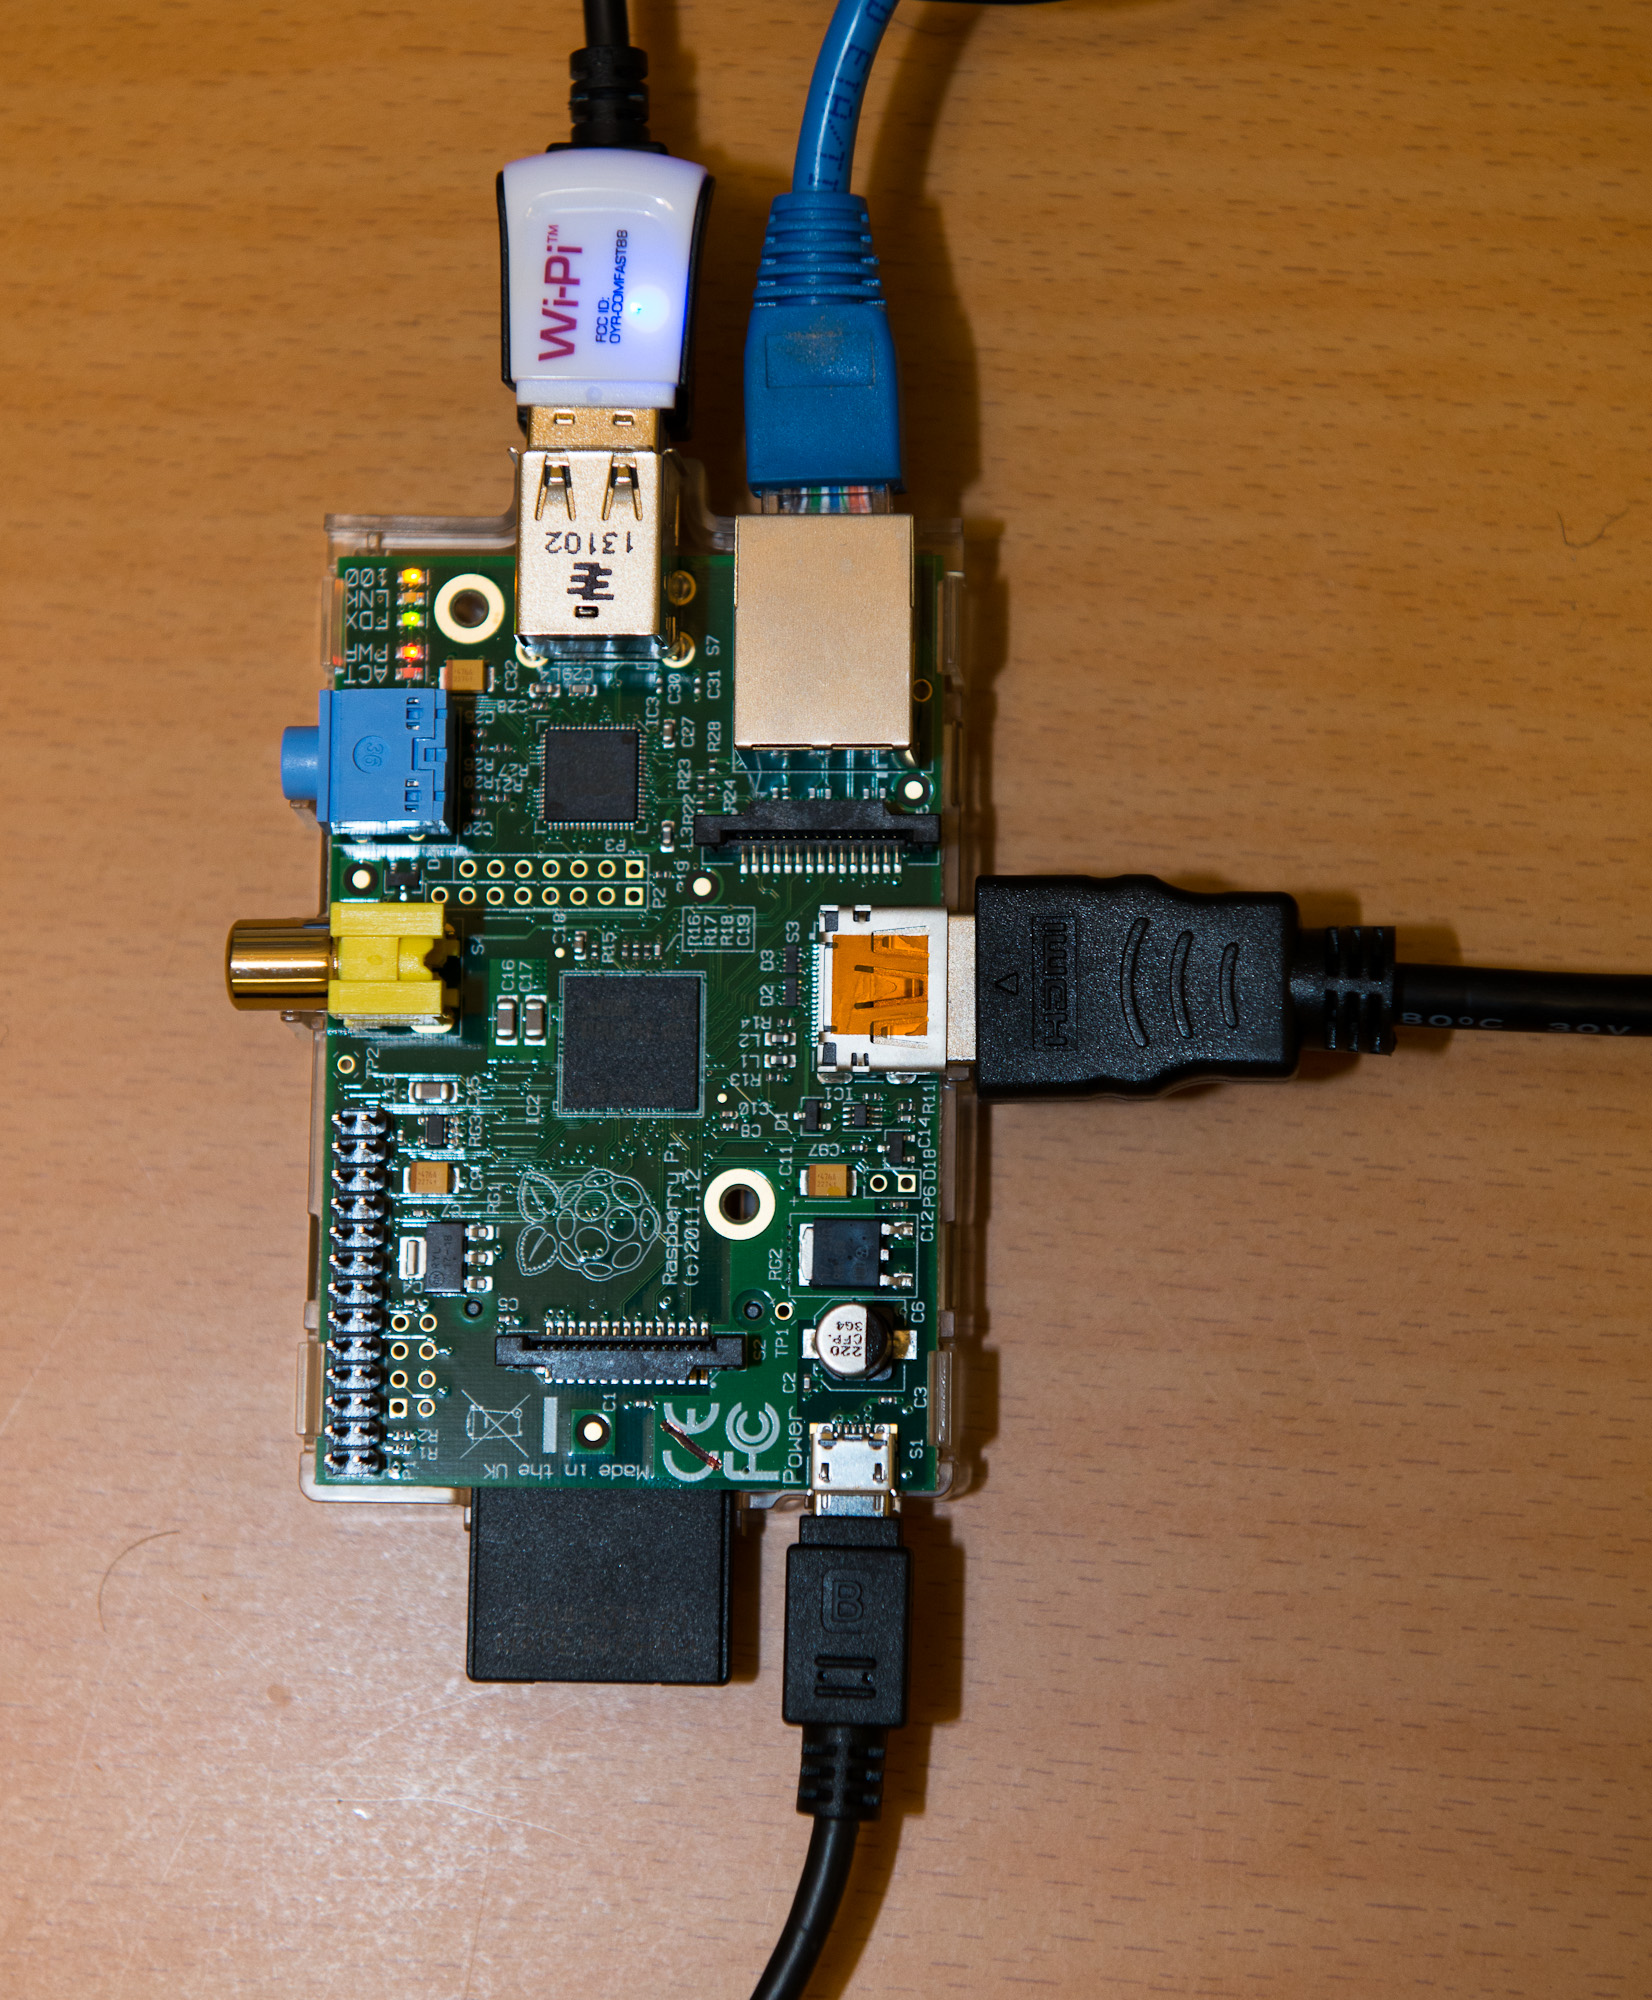
\includegraphics[width=.7\textwidth]{groundstation}
        \caption{The ground station}\label{fig:ground-station}
    \end{subfigure}%
    \begin{subfigure}{.5\textwidth}
        \centering
        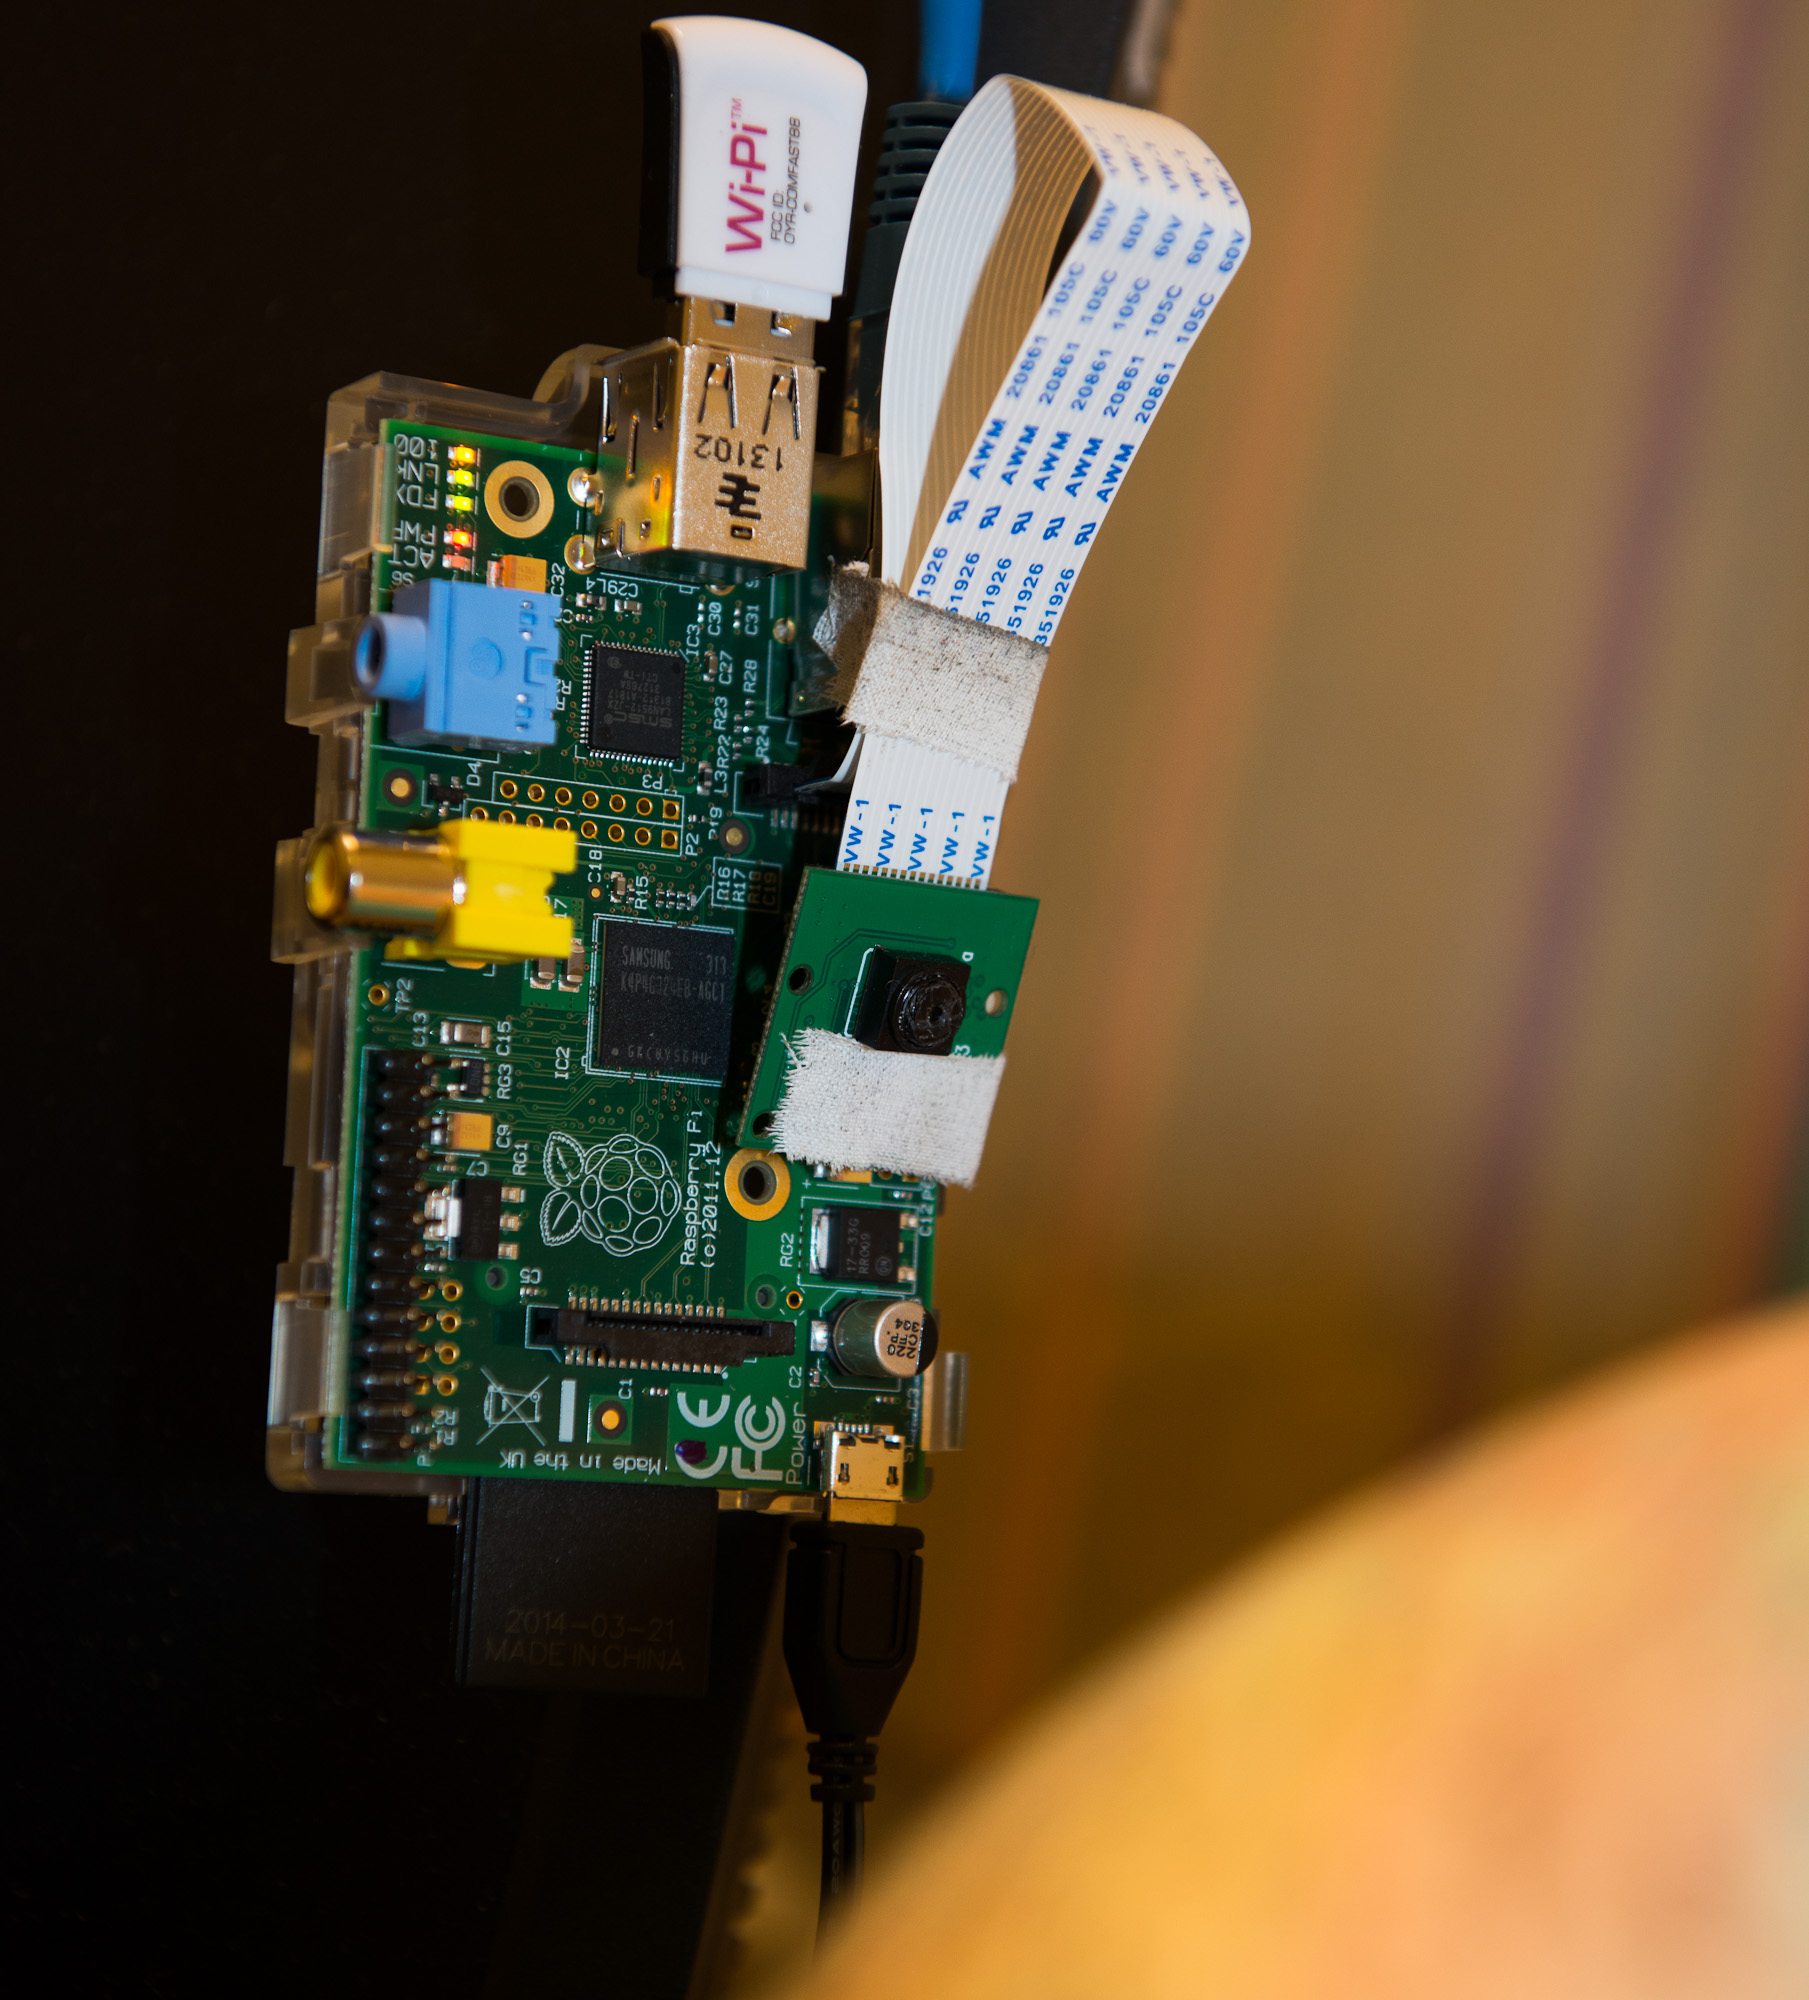
\includegraphics[width=.7\textwidth]{satellite}
        \caption{The satellite}\label{fig:satellite}
    \end{subfigure}
    \caption{The two Raspberry Pis used in the test environment}\label{fig:raspberrys}
\end{figure}

To test the code in a real environment with package loss and propagation delays, we set up a system with two Raspberry Pis, communicating over an open Wi-Fi connection. Additionally, the server was equipped with a camera, to generate payloads to send to the client. The following hardware was used:

\begin{itemize}
    \item 2 $\times$ Raspberry Pi model B
    \item 2 $\times$ Element14 Wi-Pi USB Wi-Fi dongle
    \item Element14 Raspbery Pi 5MP Camera Board
\end{itemize}

There was also one globe involved, to simulate the server being in orbit. The wireless network was hosted on the server by \texttt{hostapd}, and the server also ran a DHCP server using \texttt{dnsmasq}. Both Raspberry Pis were running Raspbian Wheezy. Both of the Raspberry Pis were like you can tell from \autoref{fig:raspberrys} also connected by Ethernet. This was merely for control purposes, to make it possible to SSH into the devices to add the code and start the tests. You can also see that the client has a HDMI connection, this was used to display the downloaded images on a monitor, as demonstrated later in \autoref{fig:test-environment}

It must be said that the code does not have to be run over Wi-Fi, it might be just as interesting for students studying the protocol to try to mount a wired \gls{mitm} attack. This could be done by utilizing a computer with two wired Ethernet interfaces, and gives you the possibility to delay packets, re-order them, drop a select few, etc. Eventually, this computer in the middle could just be used for monitoring, following the packet flow between the client and the server in real-time to better understand the protocol.


\section{Results}\label{sec:results}

The examples mentioned here run successfully in the test environment. The following is a "satellite image" taken by the server "in orbit" over Japan (\autoref{fig:test-environment}, extracted by the client using the re-assembly code given in \autoref{lst:nap-client-image}.

\begin{figure}[ht!]
\centering
    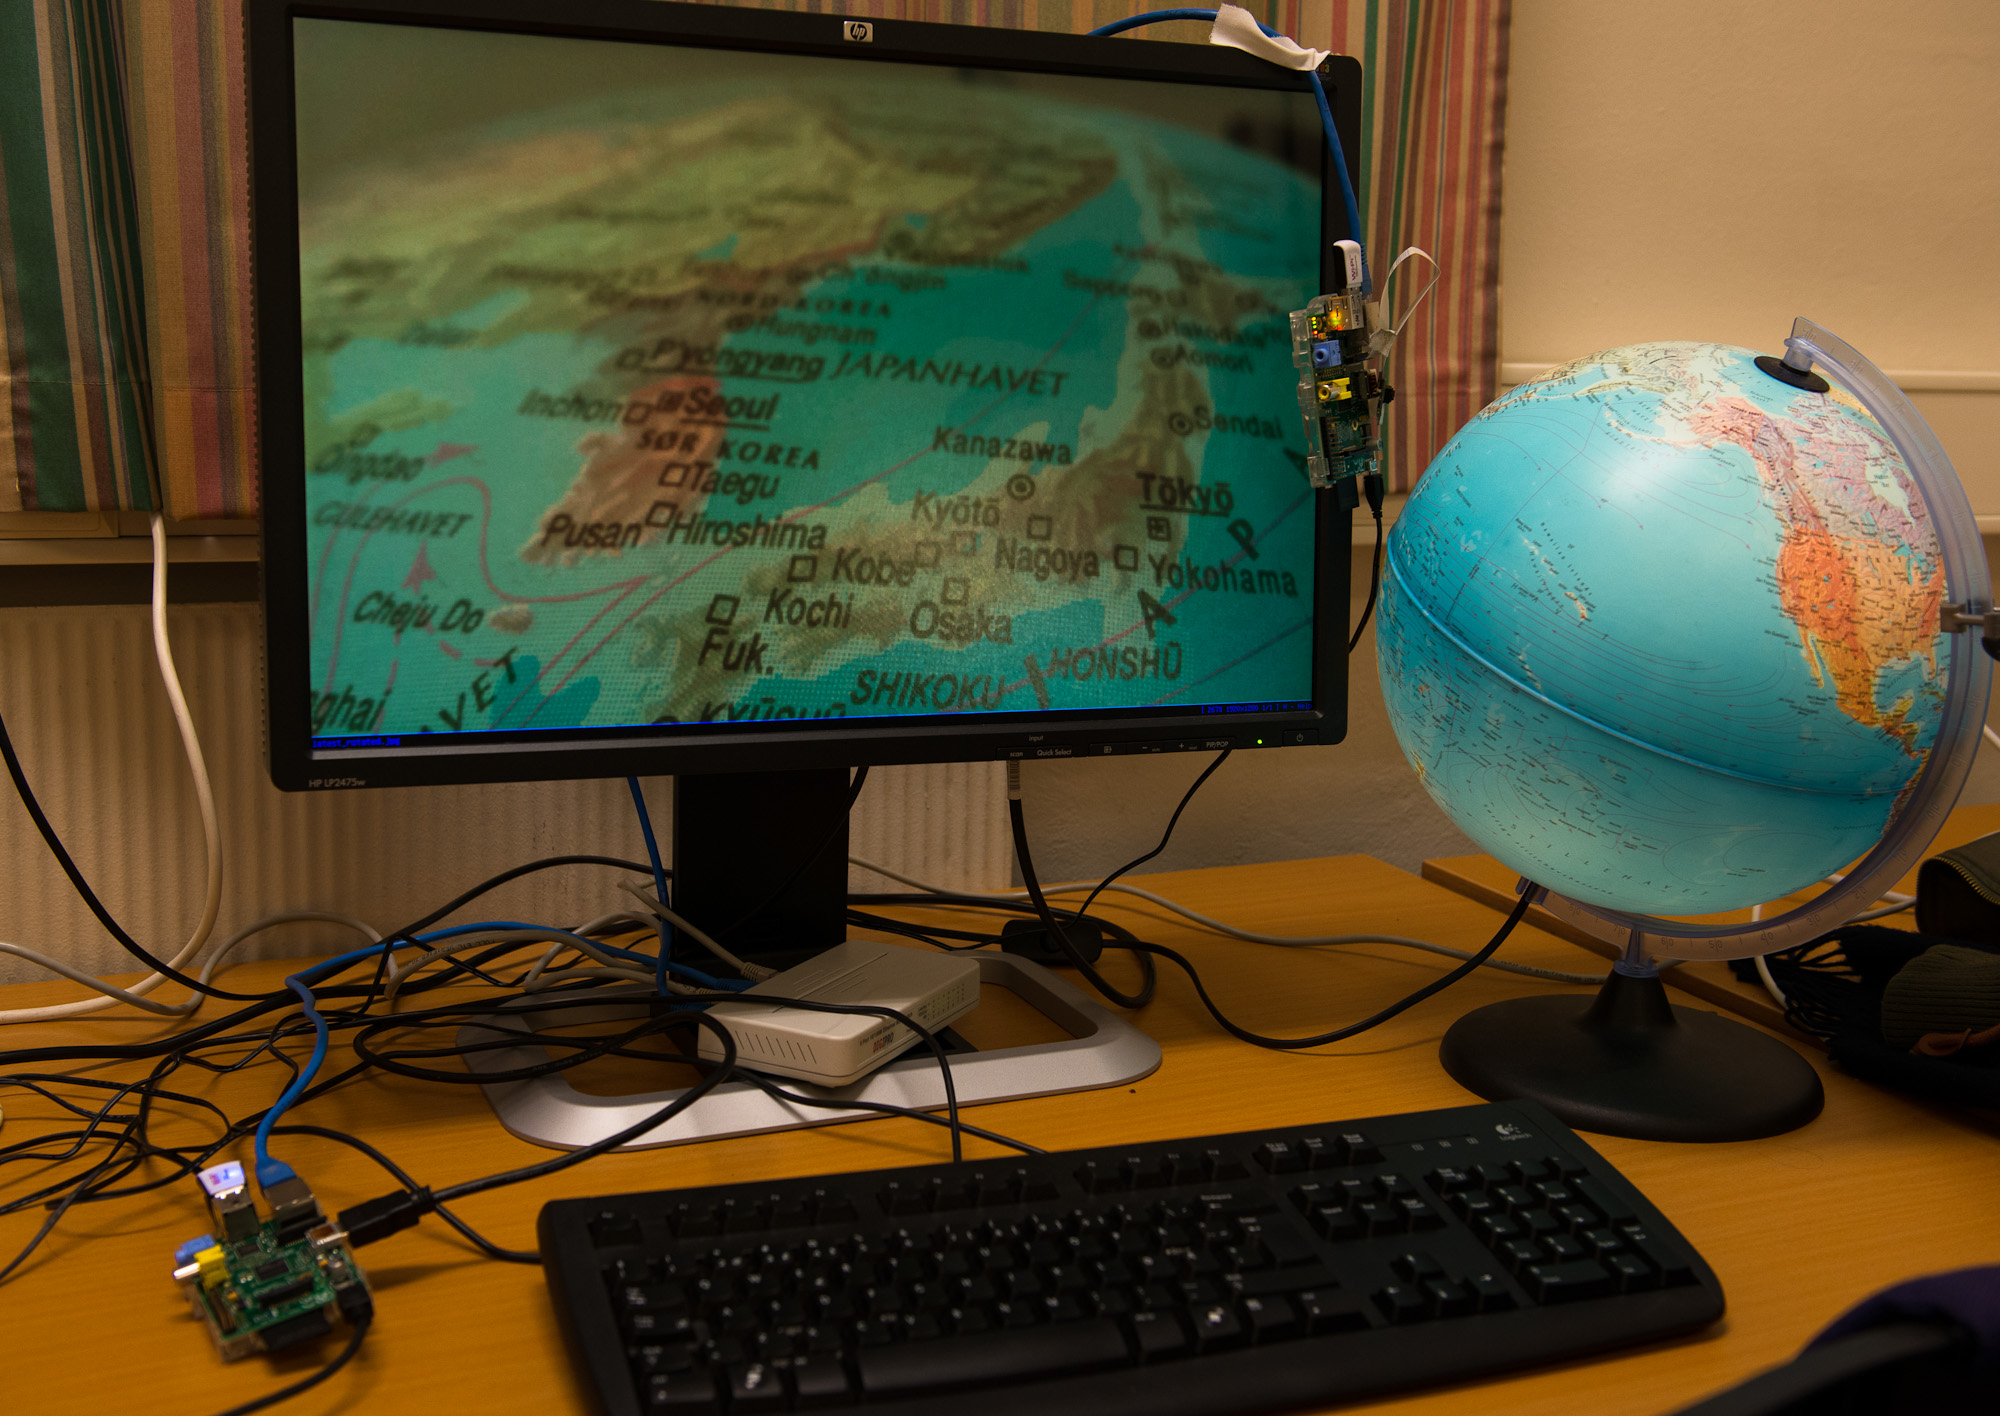
\includegraphics[width=110mm]{test-environment}
    \caption{The client displaying an image it just downloaded and re-assembled from the satellite}\label{fig:test-environment}
\end{figure}

There were some problems with executing the examples in the test environment, but the problems were not related to our code, which was frustrating. It turned out hard to configure the wireless adapters without them sporadically loosing their IP after some time. This happened irregularly on both devices, requiring either restarting the wireless interface or a full restart of the unit to get things back into a stable state. It might be that stable connectivity is more than what can be expected from a small computer costing around 200 NOK over a wireless dongle in 2014, but it was certainly worse than expected. The stability issues might be due to the wireless network being hosted on one of the Raspberry Pis, which have very limited power usage due to them being run over USB power, so it might be that the stability would have been better with a dedicated router.
